\chapter{Ores and the Miseries of Modernity}

\chapterauthor{Marc Los Huertos, Alison Hong, and ??\footnote{Statement of Contributions: Alison Hong started a provocative description of the issues with gold mining in the Philippines. Later, Los Huertos decided to put these mining activities in a geologic context and revised the fossil fuel chapter that links to development of a population dependent on high density of energy.}}

\section{Mining Metals}

\subsection{Aluminum, Copper, and Rare Earth Metals}


\subsection{Gold in the Philippines}

The Philippines had the second largest gold reserve in world and employs approximately 200,000-300,000 people, most of who work in small scale mining operations, making approximately \$5/day (Pri)[??]

Many family miners, independent miners who make up the 70-80\% from small mining operations in the country. 


Large scale: \$70 billion 2014 (HWR)

90\% smuggled illegally

2015: Gov simplified process of gaining license 

But the Phillipines on just one region that has been subjected to the demand of gold and the re-occuring environmental and human tolls from the economic demand for gold. It drove some of the worst human behaviors from massacres, poisoning and destruction of whole groups of people via slavery and colonization. Although one could argue that the conditions today in the Phillipines is much better that the mines in the Andes or Brazil in the 1800s, but we would still be confronted with a terribly injustice system. To make a difference, we need to better appreciate why are these ores found unevenly and what are the processes to extract them and finally, how are the refined products used. 


\subsection{Geology and Gold}

\subsubsection{Mining and Processing Gold}

\subsection{Mining Methods and Ecological Impacts}

\subsubsection{Large Scale Processing}

\subsubsection{Small Scale Operations}

\citet{drasch2001mt} \ldots

Working small scale in families... (Figure \ref{fig:famliymining}).

\begin{figure}[!ht]
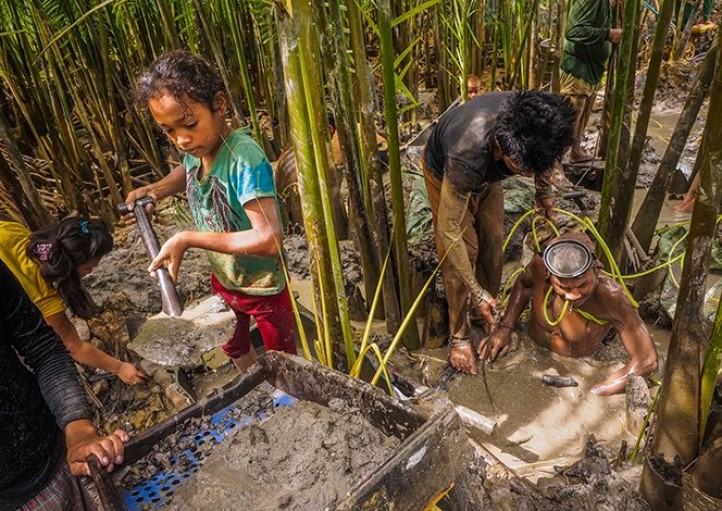
\includegraphics[width=\textwidth]{Family_Mining_Phillipines_SourceUnknwn}

\caption{Insert Caption Here: \ldots (With Permission ??).}
\label{fig:famliymining}
\end{figure}

\citep{de2016copper}

De la Torre, JB, Claveria RJ, Perez RE, Perez TR, Doronilla Al. 2016. Copper uptake by Pteris melanocaulon Fee from a Copper-Gold mine in Surigao del Norte Philippines. CRC Press LLC. 

Saludes, Mark. September 29, 2015. Hazardous Child Labor in Small-Scale Gold Mining in the Philippines. Human Rights Watch; [September 29, 2015; February 6, 2018].

\citet{santos1974mineral}

Santos G. 1974. Mineral Distribution and Geological Features of the Philippines. In: Petrascheck W.E. (eds) Metallogenetische und Geochemische Provinzen / Metallogenetic and Geochemical Provinces. /:Osterreichische Akademie der Wissenschaften Schriftenreihe der Erdwissenschaftlichen Kommission, vol 1. Springer, Vienna

Wernick, Adam. June 3, 2014. In the Philippines, underwater gold mining comes with small payoffs and big risk. PRI; [June 3, 2014; February 6, 2018]. 

\citet{drasch2001mt}

\section{Asia's Appetite for Sand}

Larson, Christina. "Asia's hunger for sand takes toll on ecology." (2018): 964-965.


%\bibliography{../references}

